\documentclass[a4paper,10pt]{jsarticle}
% 数式
\usepackage{amsmath,amsfonts}
\usepackage{bm}
% 画像
\usepackage[dvipdfmx]{graphicx}
\usepackage{here} %画像の表示位置調整用
\usepackage{type1cm}

%A4: 21.0 x 29.7cm


\begin{document}
% 有限温度におけるgap方程式
\begin{equation}
  \Delta = \dfrac{G}{2}\sum_{j} \dfrac{\Delta}{\sqrt{(\epsilon_j-\lambda)^2+\Delta^2}}\tanh(\dfrac{1}{2}\beta(\epsilon_j-\lambda))
\end{equation}
% $\Delta=0$以外の解がなくなるような温度$T_c$を求める。あ
 また、有限温度における粒子数保存の式
 \begin{equation}
  N = 2\sum_{j>0}\left\{v_j^2+(u_j^2-v_j^2)\dfrac{1}{1+\exp(\beta E_j)}\right\}
 \end{equation}
% \begin{equation}
%   \left.\begin{aligned}
%   u_i^2\\
%   v_i^2
%   \end{aligned}\right\}=
%   \dfrac{1}{2}\left(1\pm\dfrac{\epsilon_j-\lambda}{\sqrt{(\epsilon_j-\lambda)^2+\Delta^2}}\right),\quad E_i=\epsilon_i-\lambda 
% \end{equation}
% を用いて化学ポテンシャルを再計算した。

\begin{figure}[H]
  \begin{minipage}[b]{0.4\textwidth}
    \centering
    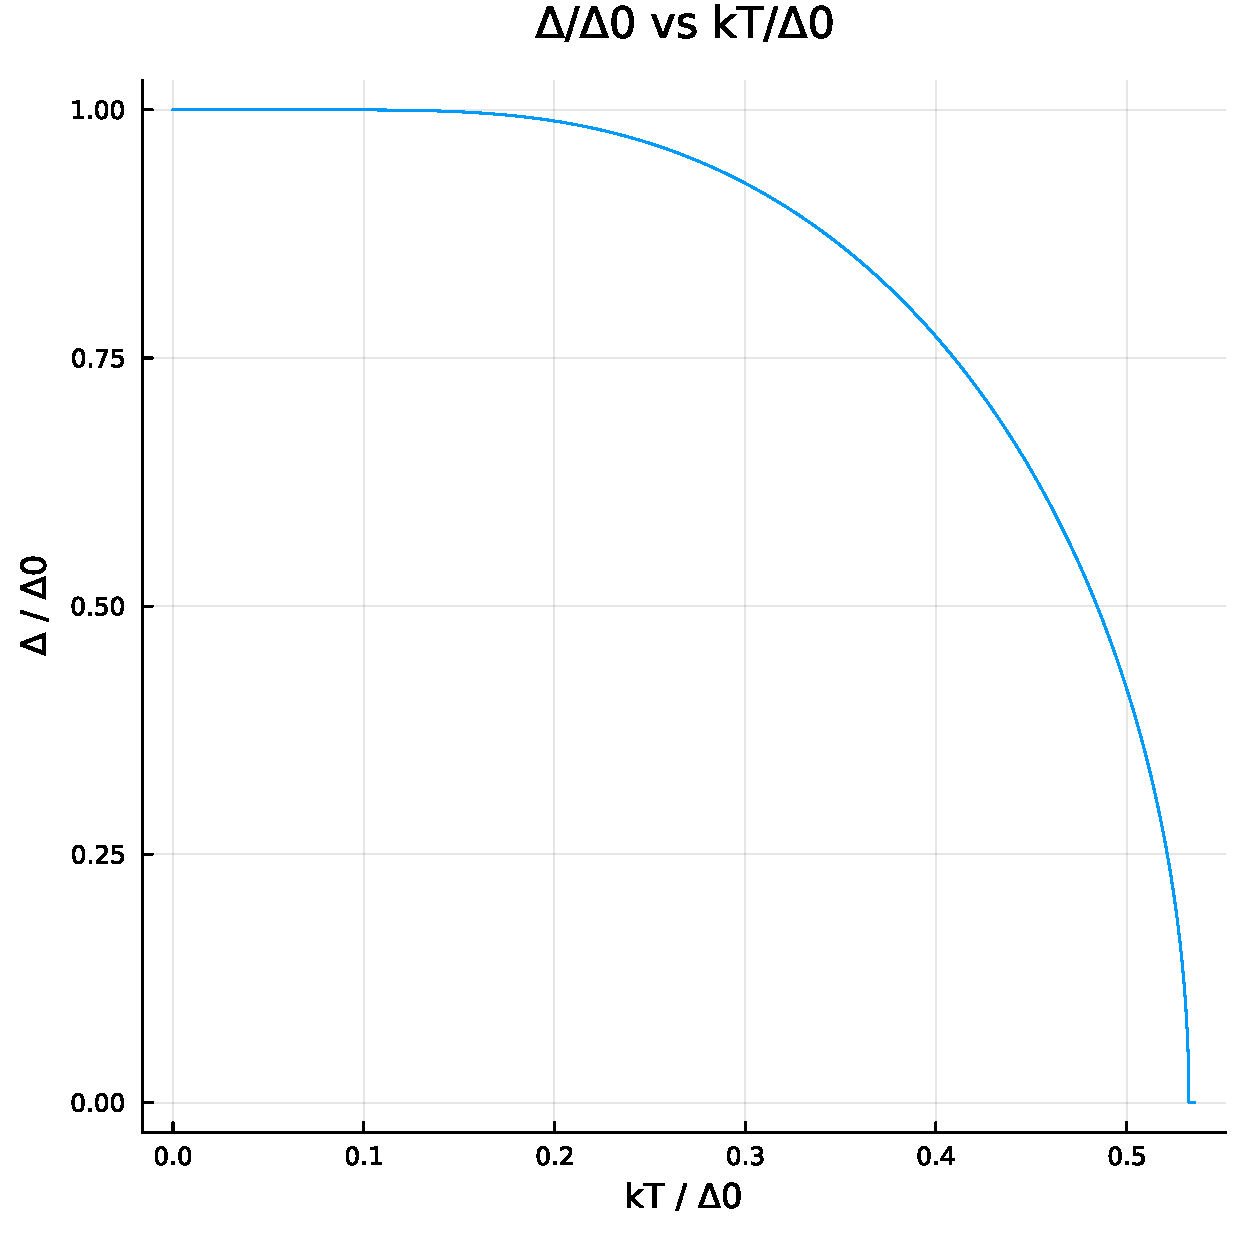
\includegraphics[width=\textwidth]{1.pdf}
    \caption{gap parametor の温度変化}
  \end{minipage}
  \begin{minipage}[b]{0.4\textwidth}
    \centering
    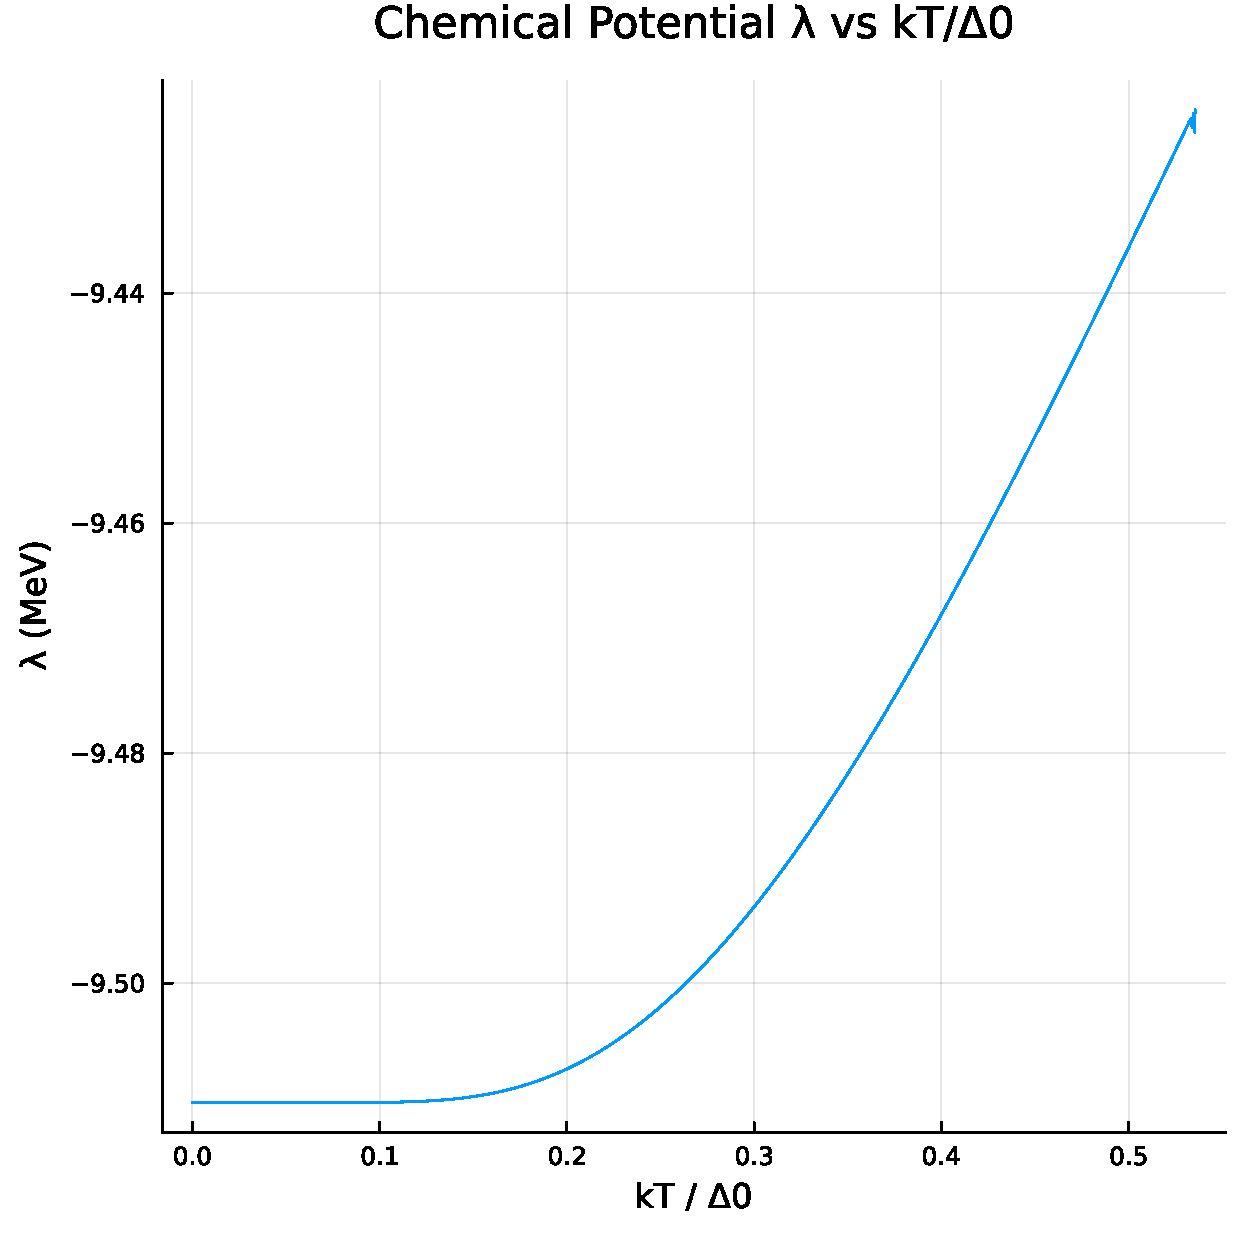
\includegraphics[width=\textwidth]{2.pdf}
    \caption{化学ポテンシャルの温度変化}
  \end{minipage}
\end{figure}
相転移が起きている点$k_B T_c =0.678$MeVから$k_B\simeq8.614\times 10^{-11}$(MeV/K)より、$T_c=7.87\times10^{9}$[K].
\begin{figure}[H]
  \begin{minipage}[b]{0.4\textwidth}
    \centering
    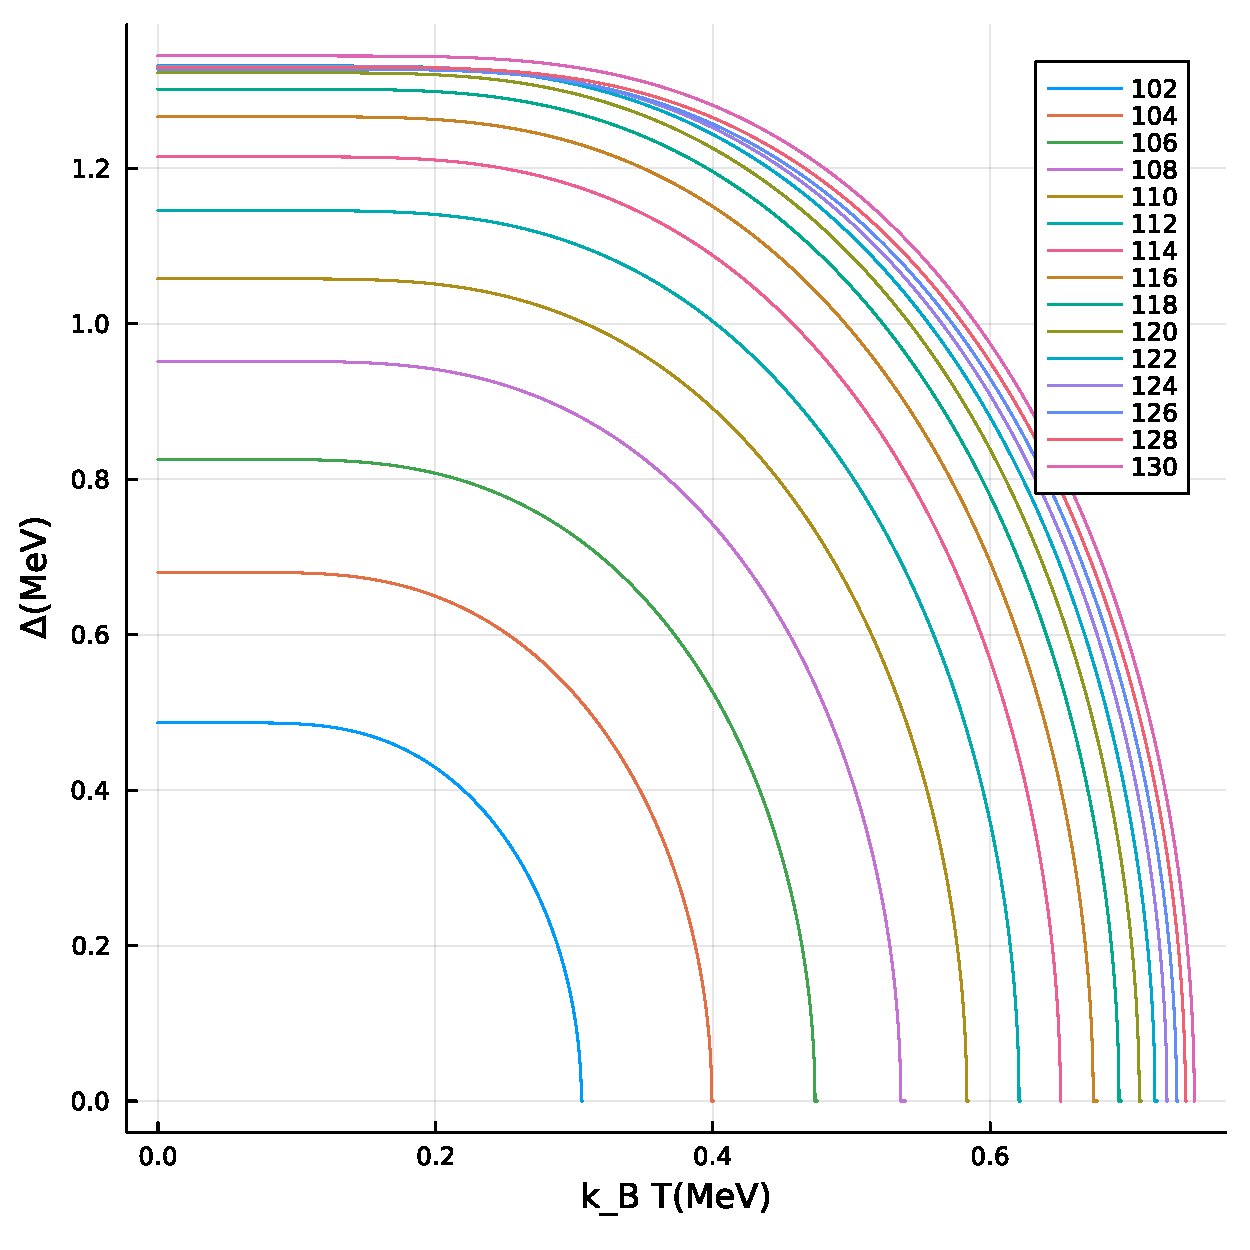
\includegraphics[width=\textwidth]{CompareFT.pdf}
    \caption{$G,\lambda$をそのまま用いた。}
  \end{minipage}
  \begin{minipage}[b]{0.4\textwidth}
    \centering
    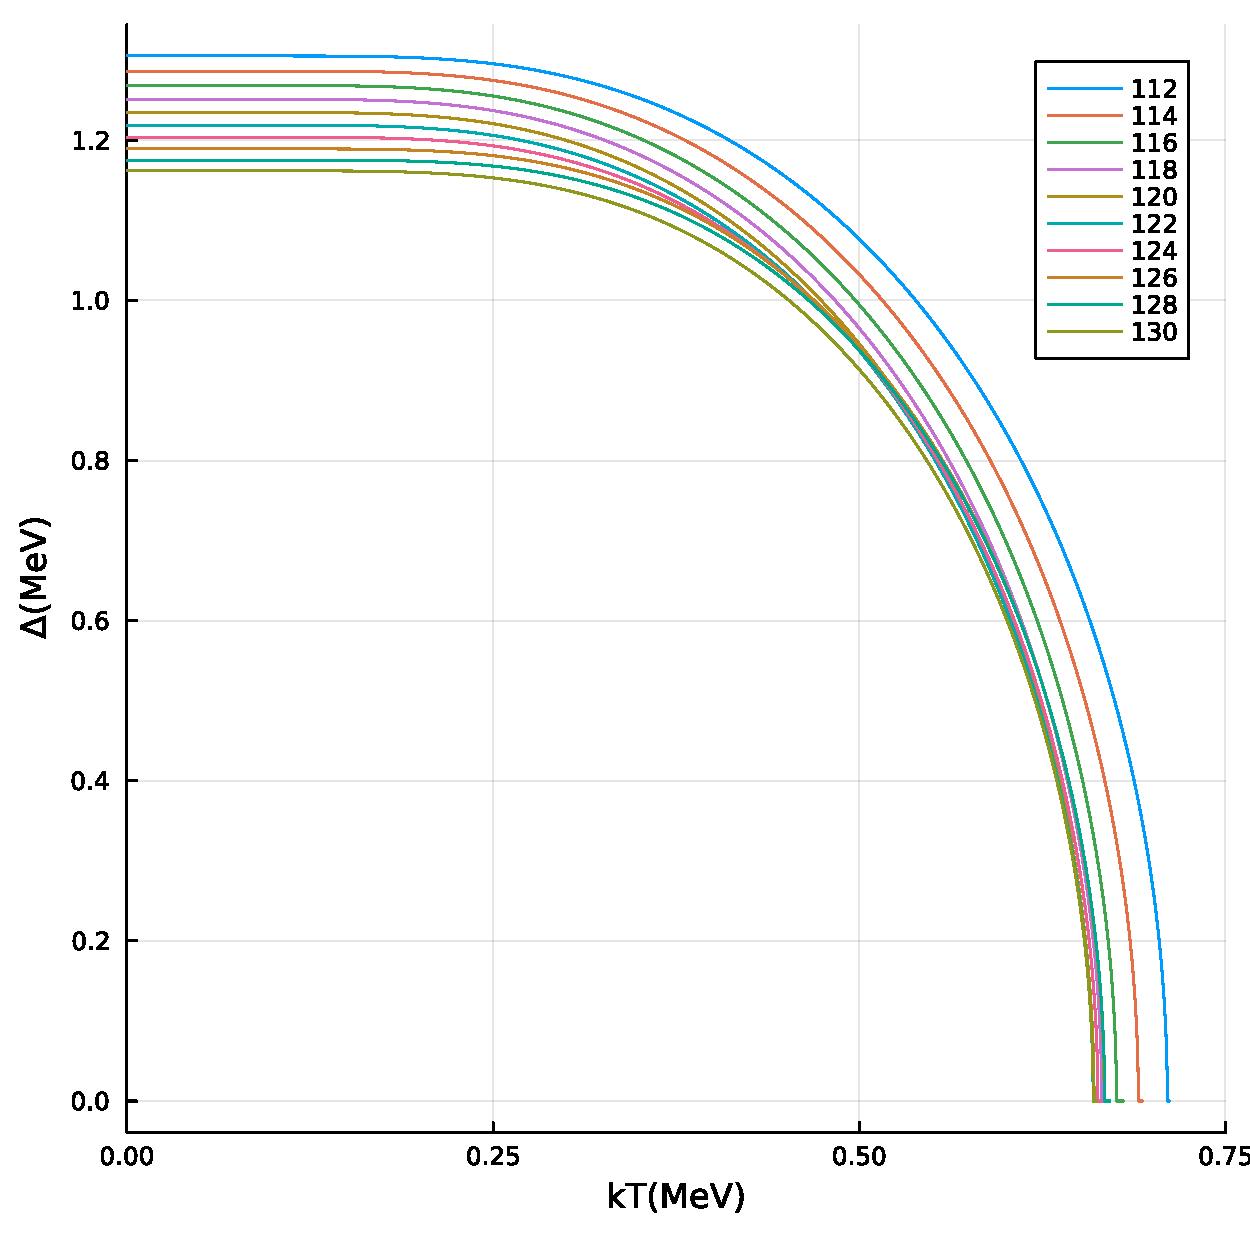
\includegraphics[width=\textwidth]{CompareFT_copy.pdf}
    \caption{$G,\lambda$を再計算した。}
    \label{fixed}
  \end{minipage}
\end{figure}
図\ref{fixed}は絶対零度のgap方程式が解けたもののみ計算対象とした。

今後
\begin{itemize}
  \item エネルギーの温度変化$\rightarrow$比熱の観察
  \item ペアリングポテンシャルの大きさ$-\dfrac{\Delta^2}{G}$ を見る
  \item エントロピーなどの熱力学的な量も計算できるのではないか?
\end{itemize}
\end{document}